\section{PIR框架细节}
\label{sec:pir-framework}
{这一段内容基本可以从专利里抄,但是得扩充一下}

本节主要讨论本文提出的基于纠删码划分的PIR协议框架细节。从设计思路触发,介绍协议框架的具体工作流程。

\subsection{框架设计}
整个框架由三层构成,分别是编码层,PIR层与解码层,其工作流程如图\ref{fig:pir-framework}所示。

\begin{figure}
    \centering
    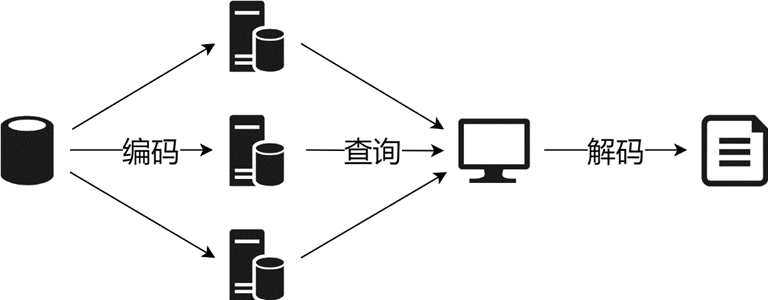
\includegraphics[width=0.8\textwidth]{figure/PIR-framework.png}
    \caption{PIR框架}
    \label{fig:pir-framework}
\end{figure}

数据库被编码后分发至多台服务器上,PIR层接收查询请求,解码层负责将PIR层的回答解码为原始数据。其中,编码与解码应满足对应关系,使用同一套编解码方案,而对于PIR层的选择则相对自由。由于前文所述原因,我们仅要求PIR层协议能够支持可验证性即可。

\subsection{框架具体流程}
框架具体执行流程如图\ref{fig:framework-protocol}所示:
\begin{figure*}
    \begin{mdframed}
        \paragraph{符号约定:} 协议包含一个客户端 $\client$ 与共$\servercount$台服务器 $\server_0,\server_1, \dots, \server_{\servercount-1}$。PIR协议层包括PIR协议$\Pi = (Setup, Query, Answer, Reconstruct)$。如果使用的PIR协议是一离线-在线PIR协议,其$Hint$被包括于$Setup$中,$Refresh$被包括与$Reconstruct$中。协议运行于包含$\dbsize$条记录的数据库$\db$上。为保证可靠性,我们期望能够容忍最多$\threshold$台服务器掉线或出错。不妨设$\servercount-\threshold$整除$\dbsize$。如此条件不能满足,可以向数据库填充空白记录直至满足。$(\servercount-\threshold, \servercount, \threshold)$纠删码方案记为$(Encode, Decode)$。

        \begin{itemize}
            \item \textbf{预处理阶段:} 服务器共同将数据库$\db$按$\servercount-\threshold$条记录大小分组,每组使用$Encode$算法编码为$\servercount$个元素,共$\frac{\dbsize}{\servercount-\threshold}$组。每组的第$i$个元素存储在第$i$台服务器上。完成之后,每台服务器应当持有大小为$\frac{\dbsize}{\servercount-\threshold}$的数据库。每台服务器使用自己的数据库运行$Setup$(包括可能存在的$Hint$)算法。
            \item \textbf{查询阶段:} 设客户端查询的记录索引为$\dbidx$。客户端分别与每台服务器运行$Query(\lfloor\frac{\dbidx}{\servercount-\threshold}\rfloor)$,服务器调用$Asnwer$给出答案,客户端调用$Reconstruct$得到共$\servercount$个答案$x_0, x_1, \dots, x_{\servercount-1}$。由于验证的缘故,其中一部分答案可能是$\bot$。
            \item \textbf{解码阶段:} 客户端调用$Decode$将共$\servercount$个答案解码为$\servercount-\threshold$条记录。并从中找到$\dbidx$对应的记录。
        \end{itemize}
    \end{mdframed}
    \caption{基于纠删码划分的PIR协议框架具体执行流程}
    \label{fig:framework-protocol}
\end{figure*}

除此之外,如果协议中的随机数是由客户端控制的,客户端可以使用完全相同的随机数与所有服务器进行交互。如此一来,客户端调用$Query(\lfloor\frac{\dbidx}{\servercount-\threshold}\rfloor)$所生成的查询可以在所有服务器处通用。这使得客户端的在线计算量绝大部分都与服务器总数无关,仅与每台服务器所持有的数据库大小有关。

\subsection{支持数据库更新}

处理数据库的增删改可以简单规约为对子数据库的增删改,其细节我们已经在第\ref{sec:handling-updates}节中讨论过。仅剩的问题是如何处理服务器的增减。在此,我们分两类情况讨论:
\begin{itemize}
    \item 修改服务器数量,不改动数据分组:在采用Reed-Solomon编码时,这种修改是平凡的。新增的服务器需要协商得到自己的子数据库,但是其他服务器的数据不需要改动。删除服务器时,不需要进行任何额外操作。
    \item 修改数据分组方式:这要求所有服务器共同重新运行预处理阶段。
\end{itemize}

